\documentclass{article}[a4paper]
\usepackage[a4paper, total={6in, 9.5in}]{geometry}
\usepackage{charter}
\usepackage{xcolor}
\usepackage{graphicx}
\usepackage{float}
\usepackage{listings}
\usepackage{tabularray}
\usepackage{amsmath}
\usepackage{amssymb}
\usepackage{enumitem}
\usepackage{tikz}
\usepackage{pgfplots}
\usepackage[hidelinks]{hyperref}

\newcommand{\extlink}{
	
\begin{tikzpicture}[scale=0.1]
		\draw[rounded corners=0.5mm, line width=0.9pt] (-1, -1) rectangle (1, 1);
		\fill[white] (0, 0) rectangle (1.3, 1.3);
		\draw[line width=0.9pt, line cap=round] (0.15, 0.15) -- (1.3, 1.3);
		\draw[line width=0.9pt, line cap=round] (0.5, 1.3) -- (1.3, 1.3) -- (1.3, 0.5);
	\end{tikzpicture}
}

\lstset{
  language=Python,
  basicstyle=\ttfamily,
  keywordstyle=\color{blue},
  commentstyle=\color{gray},
  stringstyle=\color{red},
  showstringspaces=false,
  columns=fullflexible,
  breaklines=true,
  captionpos=b,
  backgroundcolor=\color[rgb]{0.96,0.96,0.96},
  xleftmargin=6pt,
  frame=tlbr,
  framesep=6pt,
  framerule=0pt,
  aboveskip=4pt,
  morekeywords={
    % NumPy
    numpy,np,array,arange,linspace,reshape,zeros,ones,empty,full,eye,random,randn,dot,linalg,mean,std,sum,min,max,argmin,argmax,
    % Matplotlib
    matplotlib,pyplot,plt,figure,subplots,plot,scatter,bar,hist,imshow,contour,title,xlabel,ylabel,legend,axis,grid,show
  }
}

\title{
	\huge{\textbf{
		Assignment 02
	}}\\
	\Large{
		Learning from Data, Related Challenges, Classification
	}\\
	\large{\phantom{}}\\
	\large{
		submitted for
	}\\
	\LARGE{
		\textbf{EN3150 - Pattern Recognition}
	}\\
	\large{
		Department of Electronic and Telecommunication Engineering
	}
	\\
	\large{University of Moratuwa}
}

\author{
	\textbf{Udugamasooriya P. H. J.}\\
	220658U\\
	\small{Progress on \href{https://github.com/pulasthi-u/en3150-assignment02}{GitHub \extlink}}
}

\date{20 August 2025}

\allowdisplaybreaks
\setlength{\parindent}{0pt}

\begin{document}
	\maketitle

	\section{Linear Regression}

	\textbf{Question 01} The main reason is the presence of outliers.
	
	Based on the inliers, we see that the desired line is an almost horizontal one. To see why a slanted line has been produced instead of a horizontal line, we look at the behavior of the squaring function;
	\begin{figure}[H]
		\centering
		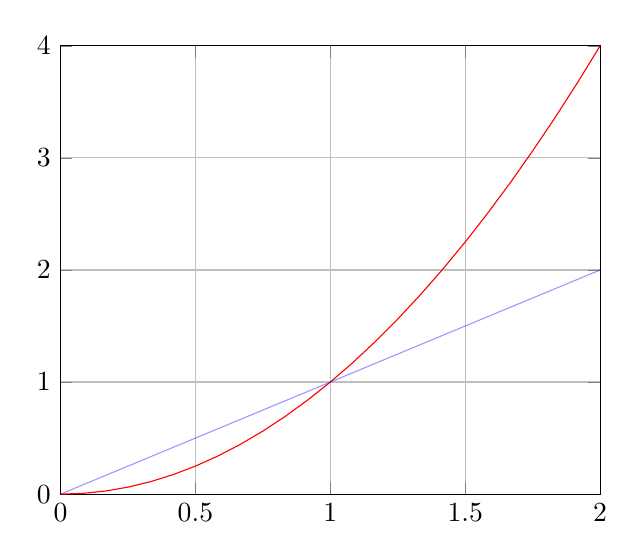
\begin{tikzpicture}
			\begin{axis}[
				xmin=0, xmax=2,
				ymin=0, ymax=4,
				grid,
			]
				\addplot[
					color=red,
					domain=0:2,
				]{x^2};
				\addplot[
					color=blue,
					opacity=0.4,
					domain=0:2,
				]{x};
			\end{axis}
		\end{tikzpicture}
		\caption{$y = x^2$}
	\end{figure}
	Note that for $|x| < 1$, $x^2 < |x| < 1$, i.e., the squares of numbers less than $1$ are less than the numbers themselves (in absolute value). This means that the squared loss function can remain small enough for prediction errors that are just slightly below $1$, but increases rapidly as it increases beyond $1$.
	\newline

	In the given situation, even though a horizontal line would give near-zero error for the inliers, the error due to outliers would be very large. It is reasonable then, that a more optimal, i.e., with a lesser mean squared error, could be achieved with a slanted line,with lesser distance between outliers and the corresponding predictions.
	\newline

	Such a line would increase the gap between the inliers and the corresponding predictions and therefore increase the loss, but \textit{not by too much}, due to the behavior of the square function. Instead, the reduction in the already-large gap between the outliers and the corresponding predictions, \textit{will} cause a \textit{rapid} decrease in the loss, \textit{exceeding} the increase in the loss due to the inliers.
	\newline
		
	\textbf{Question 02} Scheme 1.
	
	The issue we wish to mitigate is the rapid increase in loss due to outliers, while keeping the loss due to inliers significant, with the intention that a model that better fits the inliers and is not strongly affected by the outliers as described above would be preferred.
	\newline

	With Scheme 1, we do not completely neglect the effect of outliers, but significantly scale down their contribution to the loss function, so they do not dominate the loss when the loss due to the inliers is small.
	\newline

	Scheme 2 is obviously not suitable, as it amplifies the loss from outliers over inliers; minimizing such a function would require the error due to outliers to be significantly reduced, causing more slanted line to be preferred, as described in the previous problem.
	\newline

	\textbf{Question 03} why not linear regression
	\newline

	\textbf{Question 05}

	\section{Logistic Regression}

	\textbf{Question 02} The following error was encountered.
	\newline

	\textbf{Question 03} Why sagasolver bad.
	\newline
	
	\textbf{Question 04} Classification accuracy
	\newline

	\textbf{Question 05} Why liblinear better
	\newline

	\textbf{Question 06} Sagasolver accuracy
	\newline

	\textbf{Question 07} Sagasolver with feature scaling
	\newline

	\textbf{Question 08} Categorical

	\section{First and Second Order Methods for Logistic Regression}

	\textbf{Question 02} Method to initialize weights
	\newline

	\textbf{Question 03} Loss function
	\newline

	\textbf{Question 04} Newton's Method
	\newline

	\textbf{Question 05} Plots
	\newline

	\textbf{Question 06} Iterations
	\newline

	\textbf{Question 07} Convergence
\end{document}